\section{A patch-based heat equation solver}


\chapterDescription
  {
    60 minutes.
  }
  {
    Chapter \ref{chapter:quickstart}.
  }

In this section, we sketch how to realise a simple explicit heat equation
solver that is based upon patches.
The idea is that we embed a small regular Cartesian grid into each individual
spacetree leaf.
This patch is surrounded by a halo/ghost cell layer holding copies from
neighbouring patches.

\begin{center}
  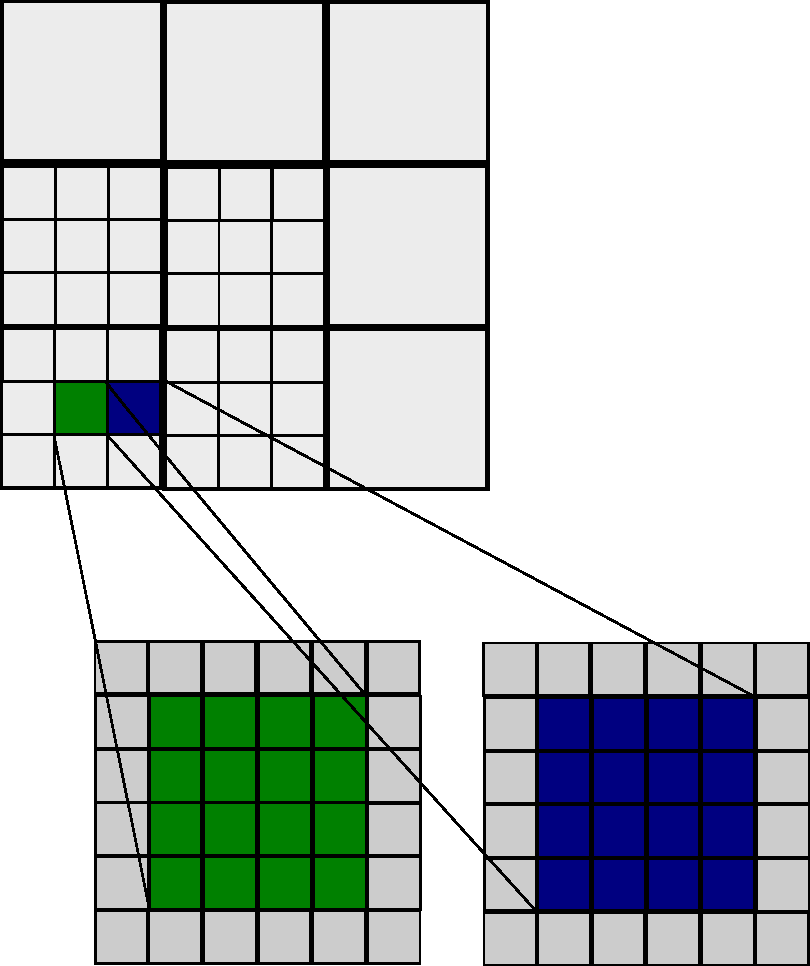
\includegraphics[width=0.4\textwidth]{22_patched-based-solver/patches.pdf}
\end{center}

In the sketch, we enbed $4\times 4$ patches into the spacetree cells.
Two cells (blue and green) are illustrated.
Each patch is surrounded by a halo layer of size one.
We will write the code to work within the patches, while the layers around the
patches will hold copies of the neighbouring patches and thus couple them.

For this endeavour, we need the toolbox \texttt{multiscalelinkedcell} that you
can download from the Peano webpage.
We assume that the whole toolbox is unzipped into a directory
\texttt{multiscalelinkedcell} which is held by your source directory.


\subsection{Preparation}

We start with the creation of a file \texttt{PatchDescription.def} in your
project's root directory. 
In our example, each patch solely shall hold one array of unknowns $u$ that are
associated to the vertices of the patch.
So each patch will have exactly $(4+2+1)^2$ unknowns (the four is the size,
there's two halo cells along each coordinate axis, and then there's finally one
more vertex than there are cells).
Besides the unknowns called $u$, we also store the position and size as well as
the level with each patch---well-aware that level and size are kind of
redundant.

\begin{code}
#include "peano/utils/Globals.h"

Packed-Type:  int;

Constant: DIMENSIONS;

/**
 * A cell description describes one individual patch of the overall grid, i.e. 
 * it holds pointers to the actual data of the patch (arrays) and its meta data
 * such as time stamps. Each unrefined node of the spacetree, i.e. each leaf, 
 * holds exactly one instance of this class. 
 */
class patchwork::records::PatchDescription {
  /**
   * Two pointers to float arrays.
   */
  parallelise persistent int     u;
  /**
   * I need level and offset to be able to determine the source and image in 
   * the adaptive case.
   */
  parallelise persistent int     level;
  parallelise persistent double  offset[DIMENSIONS];
  parallelise persistent double  size[DIMENSIONS];
};
\end{code}

Please note that $u$ is modelled as integer. 
Actually, we do not hold the data directly within the patch description but we
make the patch description hold a pointer to the actual data.
The data will be managed by Peano on the heap. 
The heap uses integers as pointers.
They are actually hash map indices.


Our system design is as follows:
\begin{itemize}
  \item Each cell holds a pointer to one \texttt{PatchDescription}.
  \item The \texttt{PatchDescription} holds a pointer to the actual patch data
  and comprises some additional meta data (such as the level).
  \item Each vertex holds $2^d$ pointers to the
  \texttt{PatchDescription} instances belonging to the adjacent cells.
\end{itemize}


Whenever we enter a cell, we can thus take its patch description, and get the
actual data from this description.
Alternatively, we can use the cell's $2^d$ adjacent vertices. 
As they know the adjacent patch descriptions, we can also get the data
associated to cell neighbours and thus befil the ghost layers, e.g.


Take the Peano description file of our project ensurte that it contains the
following lines:
\begin{code}
heap-dastgen-file: PatchDescription.def

[...]

vertex:
  dastgen-file: Vertex.def
  read vector2PowD(int): PatchIndex
  write vector2PowD(int): PatchIndex
  
[...]

event-mapping:
  name: Mapping1


event-mapping:
  name: Mapping2
  
[...]

adapter:
  name: Adapter1
  merge-with-user-defined-mapping: Mapping1
  merge-with-predefined-mapping: MultiscaleLinkedCell(PatchIndex)

adapter:
  name: Adapter2
  merge-with-user-defined-mapping: Mapping2
  merge-with-predefined-mapping: MultiscaleLinkedCell(PatchIndex)
\end{code}

Managing all the adjaceny data (making each vertex point to the right patch)
obviously is a tedious task.
The \texttt{multiscalelinkedcell} toolbox fortunately does most of the stuff for
us, if we augment each adapter with a predefined mapping, tell this mapping what
the attribute for the patch handling will be (\texttt{PatchIndex}), and augment
the vertex accordingly. 
Finally, open \texttt{Vertex.def} and augment it accordingly:

\begin{code}
#include "peano/utils/Globals.h"

Packed-Type:  int;

Constant: TWO_POWER_D;

class patchwork::dastgen::Vertex {
  /**
   * These guys are pointers to the adjacent cells. Actually, they do not point 
   * to the neighbouring cells but to the heap indices associated to these cells.
   * These heap indices reference one or several instances of PatchDescription.
   */
  expose persistent int patchIndex[TWO_POWER_D];  
  
  [...]
};
\end{code}

We run the translation process and add the toolbox directory to the PDT call:
\begin{code}
 java -jar <mypath>/pdt.jar <mypath>/project.peano-specification <mypath> \
 <mypath>/usrtemplates:<mypath>/multiscalelinkedcell
\end{code}